\documentclass[a4paper,10pt]{article}

%%%%%%%%%%%%%%%%%%%%%%%%%%%%%%%%%%%%%%%%%
% packages
%%%%%%%%%%%%%%%%%%%%%%%%%%%%%%%%%%%%%%%%%
\usepackage{graphicx}
\usepackage{url}

\usepackage[utf8x]{inputenc}

\usepackage{graphicx}
\usepackage{amssymb}
\usepackage{amsmath}
\usepackage{lineno}
\usepackage{verbatim} 

\usepackage{array,float,epsf,psfrag,eurosym,theorem}
\usepackage{amsfonts}
\usepackage{bbm}
\usepackage{mathrsfs}

\usepackage{color}
\usepackage{srcltx}


\usepackage{geometry}
\usepackage{xspace}
\usepackage{bm}
\usepackage[figtopcap,tight,nooneline]{subfigure}
\usepackage{amssymb}

%%%%%%%%%%%%%%%%%%%%%%%%%%%%%%%%%%%%%%%%%
% definitions:
%%%%%%%%%%%%%%%%%%%%%%%%%%%%%%%%%%%%%%%%%
\newcommand{\reffig}[1]{Fig.~\ref{fig:#1}}
\newcommand{\reffigs}[2]{Figs.~\ref{fig:#1},~\ref{fig:#2}}
\newcommand{\refeq}[1]{Eq. (\ref{eq:#1})}
\newcommand{\refeqs}[2]{(\ref{eq:#1}),~(\ref{eq:#2})}
\newcommand{\reftab}[1]{Tab.~\ref{tab:#1}}
\newcommand{\reftabs}[2]{Tabs.~\ref{tab:#1},~\ref{tab:#2}}

\newcommand*{\QEDA}{\hfill\ensuremath{\blacksquare}}%
\newcommand*{\QEDB}{\hfill\ensuremath{\square}}%

\DeclareMathAlphabet{\mathpzc}{OT1}{pzc}{m}{it}

\def\gz  #1{           \mbox{$\mathbf{#1}$}}
%\def\gz  #1{           \mbox{\boldmath $\mit #1$}}
%\def\gzb #1{\overline {\mbox{\boldmath $\mit #1$}}}
\DeclareMathAlphabet{\bsf}{OT1}{cmss}{bx}{n}
\def\msf  #1{           \mbox{\!\!      $\sf #1$}}
\def\Grad #1 {{\rm Grad} #1}
\def\grad #1 {{\rm grad} #1}
\def\Div {\mbox{Div}}
\def\d {\,\mbox{d}}
\def\D {\,\mbox{D}}
\def\gzh #1{\widehat  {\mbox{\boldmath $\mit #1$}}}
\newcommand{\norm}[1]{\left\lvert #1 \right\rvert}
\newcommand\normDouble[1]{\left\lVert#1\right\rVert}
\newcommand{\normXY}[1]{\lvert #1 \rvert_{2d}}
\newcommand{\dbracket}[1]{\left[\!\!\left[ #1 \right]\!\!\right]}

\def\mcl  #1{               {\cal #1}}
\def\bcl  #1{\mbox{\boldmath$\cal #1$}}
\def\cc #1{\,{\mathbbm #1}}

%%%%%%%%%%%%%%%%%%%%%%%%%%%%%%%%%%%%%%%%%
% document:
%%%%%%%%%%%%%%%%%%%%%%%%%%%%%%%%%%%%%%%%%

\parindent0pt
\begin{document}


\section{Derivation of energy and forces}
The position vector for particle $\alpha$ in Euclidean space with origin $\bsf x = \gz 0$ is denoted by
\begin{align}
\bsf x^\alpha \in  E^3.
\end{align}

In case of pair-potentials only, the total energy of the non-local quasi-continuum method is then defined as
\begin{align}
\msf E &= \sum_{A \in \mcl C} n_A \msf E_A \\
           &= \sum_{A \in \mcl C} n_A \sum_{\alpha \in \mcl C_A} \msf E^\alpha \\
           &= \sum_{A \in \mcl C} n_A \sum_{\alpha \in \mcl C_A} \sum_{\beta \in \mcl N_\alpha} \frac{1}{2} \msf E^{\alpha \beta} (\msf r^{\alpha\beta}),
\end{align}
where $\mcl C$ is the set of all clusters, $\mcl C_A$ is the set of atoms attributed to the cluster $A$, $\mcl N_\alpha$ is the set of atoms which interact with atom $\alpha$,
$\msf E^{\alpha \beta}$ is the energy of the interaction between particles $\alpha$ and $\beta$, which depends on the distance between the two particles $\msf r^{\alpha\beta}$.

Unknown displacement field is given in the FE vector-valued functional space as
\begin{align}
\gz u (\gz x) = \sum_{i \in N_{dofs}} u_i \, \gz N_i (\gz x),
\end{align}
where $\gz N_i (\gz x)$ are vector-valued shape functions.


\begin{figure}[!ht]
   \centering
    \includegraphics[angle=90,width=0.98\textwidth]{mesh_clusters.001.png.ps}
    \caption{
        Treatment of hanging nodes for the $h$\,-adaptive QC method.
    }
    \label{fig:mesh_clusters}
\end{figure}

\begin{figure}[!ht]
    \centering
    \includegraphics[angle=90,width=0.98\textwidth]{mesh_clusters_mpi.001.png.ps}
    \caption{
        An example of partition of elements and DoFs among processors. Background colour for each DoF indicate which processor owns it.
    }
    \label{fig:mesh_mpi}
\end{figure}


Gradient of the total energy with respect to the unknown DoFs will require the following
\begin{align}
\frac{\partial \msf r^{\alpha \beta}}{\partial u_i} = \frac{\partial \msf r^{\alpha \beta}}{\partial \bsf r^{\alpha\beta}} \cdot \frac{\partial \bsf r^{\alpha\beta}}{\partial u_i} = \frac{\bsf r^{\alpha\beta}}{r^{\alpha\beta}} \cdot \frac{\partial \bsf r^{\alpha\beta}}{\partial u_i}
\end{align}
with
\begin{align}
\frac{\partial \gz r^{\alpha\beta}}{\partial u_i} = \frac{\partial\left[\bsf X^\alpha + \sum_l u_l \gz N_l(\bsf X^\alpha) - \bsf X^\beta - \sum_m u_m \gz N_m(\bsf X^\beta)\right]}{\partial u_i} = \gz N_i (\gz X^\alpha) - \gz N_i (\gz X^\beta)
\end{align}

Note the non-local nature of the assembly. The contribution to the gradient vector from each cell depends not only on the values of shape functions in this cell evaluated at $\bsf X^\alpha$, but also on values of the same shape function evaluated at points $\bsf X^\beta$ within its support on possibly neighbouring cells.

\begin{align}
\frac{\partial r^{\alpha\beta}}{\partial u_i} = \frac{\bsf r^{\alpha\beta}}{\msf r^{\alpha\beta}} \cdot \left[\gz N_i (\bsf X^\alpha) - \gz N_i (\gz X^\beta) \right]
\end{align}


Rewrite the total energy in the equivalent form
\begin{align}
\msf E &= \sum_{e \in \Omega} \sum_{\alpha \in \Omega_e} \sum_{\beta \in \mcl N_\alpha} \frac{1}{2} \left[n^\alpha + n^\beta\right] \msf E^{\alpha \beta} (\msf r^{\alpha\beta}),
\end{align}
where $\Omega$ is the set of all elements, $\Omega_e$ is the set of all atoms attributed to possibly different clusters within the element $e$ and $n^\alpha$ and $n^\beta$ are weights of atoms. Atoms not associated with any clusters have weights zero.


Some of the energies $\msf E^{\alpha\beta}$ will be evaluated twice. To circumvent this, we rewrite the energy as
\begin{align}
\msf E &= \sum_{e \in \Omega} \sum_{\alpha \in \Omega_e}
\left[
\sum_{\alpha < \beta \in \mcl N_\alpha^C} \left[n^\alpha + n^\beta\right] \msf E^{\alpha \beta} (\msf r^{\alpha\beta})
+
\sum_{\beta \in \mcl N_\alpha^G} \frac{1}{2} n^\alpha \msf E^{\alpha \beta} (\msf r^{\alpha\beta})
\right],
\end{align}
where $N_\alpha^C$ is a set of all atoms interacting with atom $\alpha$ and attributed to some cluster, whereas
$N_\alpha^G$ is a set of all ``ghost'' atoms, which are not attributed to any cluster.
$N_\alpha^G \cup N_\alpha^C = N_\alpha$ and $N_\alpha^G \cap N_\alpha^C =  0$.


{\color{red}TODO}: discuss parallelization via MPI + TBB within locally owned cells. Also discuss why distributed triangulation can't be used and why each MPI core needs to know the whole geometry.


\end{document}
